\documentclass{article}
\usepackage{graphicx}				
\usepackage{mathtools}	
\usepackage{hyperref}

\begin{document}
\title{Eksam assignment: Implementing Akima spline}
\author{Jedrzej Jawor}
\date{19/06/2018}
\maketitle

\section{Introduction}
This report seeks to implement the Akima sub spline and compare it with the cubic spline.

\section{Theory}
Interpolation is a process where one constructs a smooth function to fit a set of discrete data points.
This is often done in order to approximate experimental values at points where no data is availible.
\\
A spline, S(x), is a piecewise polynomial used for interpolation between two points in a discrete data set:
\begin{equation}
\label{eq:spline}
S(x)=S_i(x), x \in [x_i,x_{i+1}],
\end{equation}
for i=[1,n-1] being the index of the tabulated points.
$S_i$ is a polynomial of order k.
\\
Splines for a discrete data set are calculated by demanding the continuity of the splines and their 
derivatives at the tabulated points \cite{Prakprog}.
\\
Multiple choices of k are possible, but their efficiency as interpolation function varies as splines are
sometimes prone to wiggling, thus reducing their usefullness as interpolating functions.

One of the more common choices is a cubic spline (k=3). Cubic splines (cplines) usually have high presicion 
but they can also be prone to wiggling if the interpolated set has a large discontinuity or outliers.
\\
\\
If higher precision near such point is desired, a sub-spline can be used. Sub splines are variaitions
 on the spline method that can be used for different purpouses.
\\
One sub spline is the Akima sub-spline (aspline).
Asplines are especially usefull for data sets with discontinuities as they wiggle much less 
than csplies. However, they come with drawbacks, sacrificing maximal differentiability by 
treating one of the coefficient as a free variable used for wiggle reduction instead of demanding continuity of 
the second derivative.
\\
The method and equations for calculating coefficients for csplines and asplines, on which the code used in this 
*project is based on, come from \cite{Prakprog}.

\section{Results and Discussion}
Using the equations for asplies and csplines from \cite{Prakprog}, an aspline and cspline for a 
manually tabulated data set is constructed.
The discrete points and the splines are shown in figure \ref{fig:acspl}. It can be seen that the akima spline 
wiggles much less that the cubic spline.

\begin{figure}[h]
\label{fig:acspl}
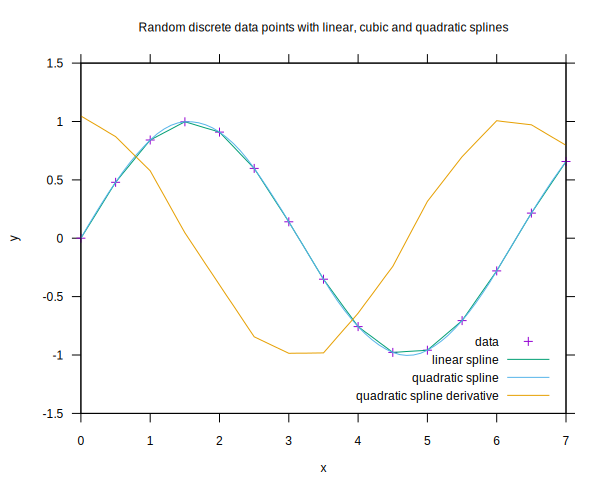
\includegraphics[width=\linewidth]{splines.pdf}
\caption{Discrete data points with the akima and cubic splines.}
\end{figure} 

Now the dervatives of the splines are found. For this purpouse, a sine function $$f(x) = sin(0.5*x)$$ 
is tabulated in discrete steps and the a- and c-splines for $f(x)$ are calutated.
\\
The derivative and the second derivative of the a- and csplines are then found. The plots of the two 
derivatives are shown in figures \ref{fig:d} and \ref{fig:d2} toghther with the analytic derivatives 
of $f(x)$.
\\
The first derivative seems to be allright, with the aspline being only a bit off compared to the cspline.
The second derivative of the aspline is not good, consistent with the theory. The cpline on the other 
hand has a very good second derivative.
\begin{figure}[h]
\label{fig:d}
\includegraphics[width=\linewidth]{dsplines.pdf}
\caption{Derivatives of aspline and cspline for $f(x)$.}
\end{figure} 

\begin{figure}[h]
\label{fig:d}
\includegraphics[width=\linewidth]{dsplines2.pdf}
\caption{Second derivatives of aspline and cspline for $f(x)$.}
\end{figure} 

Now the integration of the aspline and cspline is tested. Again using the sine function $f(x)$.
The analytical integral of $f(x)$ is:
\begin{equation}
\int_0^4 f(x) = 2.83299. 
\end{equation}

The aspline integration  yields:
\begin{equation}
\int_0^4 aspline = 2.83194. 
\end{equation}

The cspline integration  yields:
\begin{equation}
\int_0^4 cspline = 2.83203. 
\end{equation}

So the integration seems to work quite well for both the cspline and aspline (at least for a nice analytic function like sin).

\clearpage
\begin{thebibliography}{99}
\bibitem{Prakprog}
  Practical programming course book on interpolation.\\
  \emph{PrakProg: Interpolation.pdf},\\
 \url{http://86.52.112.181/~fedorov/numeric/book/interpolation.pdf}\\

\end{thebibliography}

\end{document}
